\subsection{Q10.14 data 10312021 11092021 grouped by scenario \& group}

\begin{comment}
                        EFPR        EO      EFNR     n    pvalue
(frauth, majority)  0.500000  0.500000  0.470588  17.0  1.000000
(frauth, minority)  0.300000  0.700000  0.460000  25.0  0.013221
(icu, majority)     0.593750  0.406250  0.625000  16.0  0.266715
(icu, minority)     0.400000  0.600000  0.525000  20.0  0.861804
(rent, majority)    0.525000  0.475000  0.400000  20.0  0.846517
(rent, minority)    0.263158  0.736842  0.447368  19.0  0.040045
\end{comment}

\begin{table}[h]
    \centering
    \begin{tabular}{|c|c|c|c|c|c|c|}
        \hline
        scenario & group & EFPR & EO & EFNR & n & p-value\\
        \hline
        frauth & majority & 0.500 & 0.500 & 0.471 & 17.0 & 1.000\\
		frauth & minority & 0.300 & \textbf{0.700} & 0.460 & 25.0 & \textbf{0.013}\\
		icu & majority & \textbf{0.594} & 0.406 & \textbf{0.625} & 16.0 & 0.267\\
		icu & minority & 0.400 & \textbf{0.600} & \textbf{0.525} & 20.0 & 0.862\\
		rent & majority & \textbf{0.525} & 0.475 & 0.400 & 20.0 & 0.847\\
		rent & minority & 0.263 & \textbf{0.737} & 0.447 & 19.0 & \textbf{0.040}\\
		
        \hline
    \end{tabular}
    \caption{Grouped by scenario group}
    \label{tab:my_label}
\end{table}
\begin{figure}[h]
    \centering
    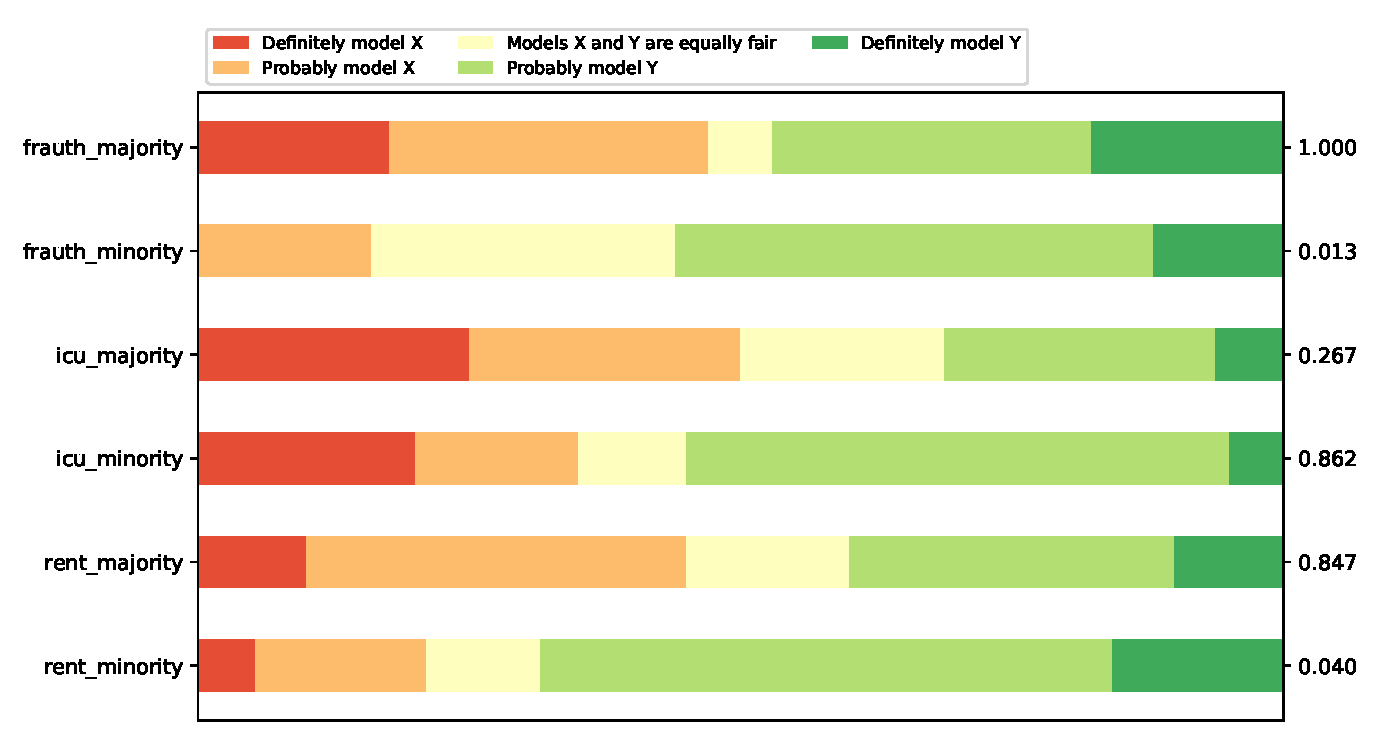
\includegraphics[width=0.8\textwidth]{figures/Q10.14/10312021_11092021/Q10.14_scenario_group.pdf}
    \caption{Grouped by scenario \& group}
    \label{fig:my_label}
\end{figure}
